\documentclass[utf8,14pt, coursreport]{G7-32}
% masterthes -- диссертация магистра
% diploma -- дипломная работа инженера
% bachelor -- квалификационная работа бакалавра
% coursreport -- курсовая работа
% projreport -- курсовой проект по дисциплине
% appreport -- отчет о прикладных научных исследованиях
% scireport -- отчет о научно-исследовательской работе
% report -- отчёт (по практике)
\usepackage[utf8]{inputenc}
\usepackage[english,russian]{babel}
\usepackage{epstopdf}
%\usepackage{bookmark}
\usepackage{titletoc}

\usepackage[colorlinks=true, citecolor=blue, bookmarksopen=true]{hyperref}

% additional packages
%\usepackage{subcaption}
%\usepackage{float}
%\usepackage{rotating}
%\usepackage{multirow}
%\usepackage{mdwlist}
\usepackage{textcase}
\usepackage{array}
\usepackage{graphicx}


% avsolov: 2014-11-13: Не используйте \url{} внутри BIB!
% Это приводит к ошибке: TeX capacity exceeded, sorry [input stack size=5000]
% И вообще в отчете по ГОСТ нет необходимости в тегах \url{}.
%\usepackage{hyperref}

\TableInChapter % таблицы будут нумероваться в пределах раздела
\PicInChapter   % рисунки будут нумероваться в пределах раздела
\EqInChapter    % формулы будут нумероваться в пределах раздела

% Определяем заголовки для титульной страницы
%% Полное название организации
\NirOrgLongName{{\small Министерство образования и науки Российской Федерации\\
 Федеральное государственное бюджетное образовательное учреждение высшего образования}\\ <<Петрозаводский государственный университет>>\\
Физико-технический институт\\
Кафедра физики твердого тела}

\NirAuthor{\signfield{Автор работы:\newline студент группы 21312}{В.\,Б.\,Охотников}}

\NirSupervisor{\signfield{Научный руководитель:\newline канд.\,физ.-мат.\,наук, доцент}{И.\,В.\,Климов}}

%\NirYear{2015} %% год отчёта; если закомментировано, ставится текущий год
\NirTown{Петрозаводск} %% город, в котором написан отчёт


%%%%%%%<------------- НАЧАЛО ДОКУМЕНТА

\begin{document}
\usefont{T2A}{ftm}{m}{} %%% Использование шрифтов Т2 для возможности скопировать текст из PDF-файлов.

\frontmatter %%% <-- это выключает нумерацию ВСЕГО; здесь начинаются ненумерованные главы типа Исполнители, Обозначения и прочее

% \NirTitle{ПРАВИЛА ОФОРМЛЕНИЯ ВЫПУСКНЫХ КВАЛИФИКАЦИОННЫХ РАБОТ}{09.04.01 ``Информатика и вычислительная техника''} %%% Название работы, доп.параметр - направление подготовки; <-- генерация титульного листа

\NirTitle{РАЗРАБОТКА СИСТЕМЫ МОНИТОРИНГА И ПРОГНОЗИРОВАНИЯ ПОТРЕБЛЕНИЯ ЭЛЕКТРОЭНЕРГИИ В ЭЛЕКТРИЧЕСКИХ СЕТЯХ}{} %%% Название работы, доп. параметр -- вид отчета <-- генерация титульного листа

\Referat %% Реферат отчёта, не более 1 страницы

Работа содержит \totalpages{}~с., \totalfigures{}~рис., \totaltables{}~табл., \totalbibs{}~источника.

Ключевые слова:
\begin{itemize}
\item АСКУЭ
\item Клиент
\item Сервер
\item УСПД
\item Принципиальная схема
\item USART
\item CAN
\item Ethernet
\end{itemize}

\tableofcontents

\iffalse
% Если требуется раздел "Нормативные ссылки"
\NormRefs

В данной работе использованы ссылки на следующие стандарты:

ГОСТ 2.105-95 Единая система конструкторской документации. Общие требования к текстовым документам.

ГОСТ Р 7.0.5-2008 Система стандартов по информации, библиотечному и издательскому делу. Библиографическая ссылка. Общие требования и правила составления.

ГОСТ Р 7.0.12-2011 Система стандартов по информации, библиотечному и издательскому делу. Библиографическая запись. Сокращение слов и словосочетаний на русском языке. Общие требования и правила.

ГОСТ 7.1-2003 Система стандартов по информации, библиотечному и издательскому делу. Библиографическое описание документа. Общие требования и правила составления.

ГОСТ 7.9-95 (ИСО 214-76) Система стандартов по информации, библиотечному и издательскому делу. Реферат и аннотация. Общие требования.

ГОСТ 7.32-2001 Система стандартов по информации, библиотечному и издательскому делу. Отчет о научно-исследовательской работе. Структура и правила оформления.

ГОСТ 8.417-2002 Государственная система обеспечения единства измерений. Единицы величин.

ГОСТ Р 15.011-96 Система разработки и постановки продукции на производство. Патентные исследования. Содержание и порядок проведения.

ГОСТ 9327-60 Бумага и изделия из бумаги. Потребительские форматы.
\fi


% Если требуется раздел "Обозначения и сокращения"
\Abbreviations

\begin{description}
\item[ПО] Программное обеспечение.
\item[МК] Микроконтроллер.
\item[УСПД] Устройство сбора и передачи данных.
\item[Сервер] Обслуживающее устройство в системах автоматической обработки информации.
\item[Клиент] УСПД, обрабатывающий и передающий данные на сервер с различных датчиков.
\end{description}


% Введение
\Introduction
Автоматизация сбора, обработки и выдачи информации в настоящее время широко используется в самых различных сферах человеческой деятельности. Можно выделить одну из таких целей автоматизации, как повышение качества управления объектами и процессами за счет оперативного предоставления операторам информации в требуемые сроки и форме, удобной для анализа. Также автоматизация способствует уменьшению влияния человеческого фактора и, как следствие, снижение вероятности аварий. Электрические сети ~--- один из объектов внедрения автоматизированных систем.

В связи с тем, что все процессы, возникающие в электросетях, протекают мгновенно и могут быть только зафиксированы, но не измерены напрямую, задача определения показателей качества электрической энергии не является простой. Расчитывать и выдавать объективное заключение необходимо только по статистически обработанным результатам. Очевидно, что для точного определения показателей качества электрической энергии необходимо непрерывно осуществлять наблюдение, выполнять большой объем измерений, причём с очень высокой скоростью, а также параллельно выполнять математическую и статистическую обработку получаенных данных.\cite{qualitymonitor}

Целью данной работы является разработка контроллера, способного получать данные о состоянии электрических сетей с последующей передачей на удаленный сервер.

\mainmatter %% <-- это включает нумерацию глав и секций в документе ниже


\chapter{ЛИТЕРАТУРНЫЙ ОБЗОР}

\section{Мониторинг электрических сетей}

Система \textbf{АСКУЭ --- Автоматизированная Система Коммерческого Учета Электроэнергии}, направлена на обеспечение контроля работы всего энергетического оборудования, а также комплексный и одновременно технический учет электроэнергии. Данная система разработана в целях применения на промышленных предприятиях, электростанциях и снабжающих электроэнергией организациях. В основе построения данной системы лежит связь счетчика-коммуникатора с другими подключенными к нему счетчиками, а также непосредственно с центрально управляющим сервером, который принимает всю информацию, идущую от счетчиков. Большим плюсом данной системы является то, что счетчик-коммуникатор заменил собой многие устройства, используемые до этого \cite{ascaepinfo}.

АСКУЭ является является специальной системой автоматизированного управления электроснабжением, в состав которой входят только информационные функции, а именно:
\begin{itemize}
\item централизованный контроль и измерение технологических параметров электроснабжения;
\item косвенное измерение параметров электроснабжения (технико-экономических показателей, внутренних переменных);
\item обощенная оценка и прогноз состояния автоматизированного технологического комплекса и его оборудования;
\item подготовка и передача данных в смежные и вышестоящие системы управления (бухгалтерия, плановый отдел);
\item удаленное управление объектами электроэнергохозяйства; формирование и выдача
данных оперативному персоналу;
\end{itemize}

Статегические цели содержания системы:
\begin{itemize}
\item повышение оперативности работы с заказчиками;
\item своевременное выявление спорных ситуаций;
\item целенаправленное ведение процесса энергоснабжения и обеспечения смежных и вышестоящих систем управления оперативной и достоверной информацией;
\end{itemize}

\section{Технологии передачи данных}

Существует множество различных технологии передачи данных, которые могут использоваться в УСПД. Каждая технология имеет свои достоинства и недостатки. Поскольку заранее не известно в каких условиях будет эксплуатироваться УСПД, необходимо комбинировать различные технологии передачи данных в одном устройстве. Таким образом можно добиться повышенной надежности работы с точки зрения доставки данных до сервера. Существует две большие категории технологии передачи данных, которые различаются средой передачи, а именно:
\begin{itemize}
\item проводные;
\item беспроводные
\end{itemize}

\subsection{Семейство проводных технологий Ethernet}

\textbf{Ethernet} (от лат. aether --- эфир) ~--- пакетная технология передачи данных преимущественно локальных компьютерных сетей. Стандарты Ethernet определяют проводные соединения и электрические сигналы на физическом уровне, формат кадров и протоколы управления доступом к среде — на канальном уровне модели OSI. Ethernet в основном описывается стандартами IEEE группы 802.3. Ethernet стал самой распространённой технологией ЛВС в середине 90-х годов прошлого века, вытеснив такие устаревшие технологии, как Arcnet, FDDI и Token ring\cite{ethernetinfo}.

В зависимости от скорости передачи данных и передающей среды существует несколько вариантов технологии. Независимо от способа передачи стек сетевого протокола и программы работают одинаково практически во всех перечисленных вариантах. Рассмотрим лишь небольшую часть модификации (таблица \ref{ethernettable}), которые могут быть потенциально применены для данной работы:

\begin{table}[h!]
\caption{Разновидности модификации стандарта Ethernet \cite{ethersite2}}
\label{ethernettable}
\begin{tabular}{|c|m{30mm}|p{90mm}|}
\hline
Модификация & Пропускная способность & Описание\\
\hline
10BASE-T & 10 Мбит/с & Для передачи данных используется 4 провода кабеля витой пары (две скрученные пары) категории-3 или категории-5. Максимальная длина сегмента 100 метров.\\
\hline
100BASE-TX & 100 Мбит/с & Задействована витая пара категории 5, фактически используются только две неэкранированные пары проводников, поддерживается дуплексная передача данных, расстояние до 100 м.\\
\hline
100BASE-T2 & 100 Мбит/с & Cтандарт, использующий витую пару категории 3. Задействованы только две пары проводников. Поддерживается полный дуплекс, когда сигналы распространяются в противоположных направлениях по каждой паре. Скорость передачи в одном направлении — 50 Мбит/с.\\
\hline
100BASE-T4 & 100 Мбит/с & Cтандарт, использующий витую пару категории 3. Задействованы все четыре пары проводников, передача данных идёт в полудуплексе.\\
\hline
1000BASE-T & 1000 Мбит/с & Стандарт, использующий витую пару категорий 5e. В передаче данных участвуют 4 пары. Скорость передачи данных — 250 Мбит/с по одной паре. Используется метод кодирования PAM5, частота основной гармоники 62,5 МГц. Расстояние до 100 метров\\
\hline
\end{tabular}
\end{table}

%\begin{itemize}
%\item 10BASE-T, IEEE 802.3i --- для передачи данных используется 4 провода кабеля витой пары (две скрученные пары) категории-3 или категории-5. Максимальная длина сегмента 100 метров.;
%\end{itemize}

\newpage

\subsection{Система мобильной связи GSM}

\textbf{GSM} (от названия группы \textit{Groupe Special Mobile}, позже переименован в Global System for Mobile Communications) ~--- глобальный стандарт цифровой мобильной сотовой связи, с разделением каналов времени (TDMA) и частоте (FDMA)\cite{gsmwiki}.

В стандарте определены 4 диапазона частот: 850 МГц, 900 МГц, 1800 МГц, 1900 МГц. В Европе и Азии используется два диапазона: 900 и 1800 МГц. Сравнительная характеристика представлена в таблице \ref{gsmtable}.

\begin{table}[h!]
\caption{характеристика диапазонов GSM, используемых в Европе и Азии\cite{gsmchar}}
\label{gsmtable}
	\begin{tabular}{|m{70mm}|m{40mm}|m{40mm}|}
	\hline
	Характеристики & GSM-900 & GSM-1800\\
	\hline
	Рабочий диапазон BTS-MS, МГц & 935-960 & 1805-1880\\
	\hline
	Рабочий диапазон MS-BTS, МГц & 890-915 & 1710-1785\\
	\hline
	Ширина радиоканала, кГц & $200*2$ & $30*2$\\
	\hline
	Макс. мощность MS, Вт & 0,8-8 & 0,25-4 \\
	\hline
	\end{tabular}
\end{table}

GSM обеспечивает поддержку следующих услуг:
\begin{itemize}
\item услуги передачи данных (синхронный и асинхронный обмен данными, в том числе пакетная передача данных — GPRS);
\item передача речевой информации;
\item передача коротких сообщений (SMS);
\item передача факсимильных сообщений;
\end{itemize}

\newpage

\subsection{Wi-Fi}

В качестве еще одной технологии обмена данными между разрабатываемым контроллером и удаленным сервером, была выбрана технология беспроводных сетей на базе стандарта IEEE 802.11. Использование данной технологии в УСПД значительно расширяет область размещения устройства в здании, а значит, повышает гибкость системы в целом.

\textbf{Wi-Fi} является торговой марки Wi-Fi Alliance. Аббревиатура Wi-Fi произошла от английского словосочетания Wireless Fidelity, которое переводится как <<беспроводное качество>> или <<беспроводная точность>>. В настоящее время развивается целое семейство стандартов передачи цифровых потоков данных по радиоканалам.

IEEE 802.11n – самый передовой коммерческий WiFi-стандарт, на данный момент, официально разрешенный к ввозу и применению на территории РФ. В 802.11n используются частотные каналы в частотных спектрах WiFi 2.4GHz и 5GHz. Совместим с 11b/11a/11g. Хотя рекомендуется строить сети с ориентацией только на 802.11n, т.к. требуется конфигурирование специальных защитных режимов при необходимости обратной совместимости с устаревшими стандартами\cite{wifistandarts}.

Сам стандарт WiFi 802.11n вышел 11 сентября 2009 года.
Поддерживаются частотные каналы WiFi шириной 20MHz и 40MHz (2x20MHz).
Используемая радиочастотная технология: OFDM.
Используется технология OFDM MIMO (Multiple Input Multiple Output) вплоть до уровня 4х4 (4хПередатчика и 4хПриемника). При этом минимум 2хПередатчика на Точку Доступа и 1хПередатчик на пользовательское устройство.

В данной работе предполагается, что с помощью Wi-Fi соединения можно будет получать данные от разрабатываемого контроллера на мобильные устройства, в тех местах, где проводное соединение отсутствует. Также рассматривается возможность использовани местных беспроводных корпоративных сетей для отправки пакетов на сервер по сети Интернет.

\newpage

\section{Многофункциональный трехфазный счетчик электрической энергии <<Меркурий 230 ART-03>>}

<<Меркурий 230>> относится к электронным (цифровым) счетчикам электроэнергии. В таких счетчиках на вход измерительного элемента поступает переменный ток и напряжение для получения на выходе импульсов, число которых пропорционально измеряемой активной энергии. В качестве счетного механизма служит электронное или электромеханическое устройство, которое включает в себя дисплей и запоминающее устройство\cite{mercinfo1}. 

«Меркурий 230» используется для учета энергии (активной, реактивной) и мощности в трехфазных сетях переменного тока. Учет может проходить в одном или двух направлениях в трех или четырех проводных сетях с частотой 50 Гц с использованием измерительных трансформаторов или непосредственно с возможностью тарифного учёта по зонам суток, учёта потерь и передачи измерений и накопленной информации об энергопотреблении по цифровым интерфейсным каналам\cite{mercinfo2}.

\begin{figure}[h]
	\label{mercury}
	\centering
		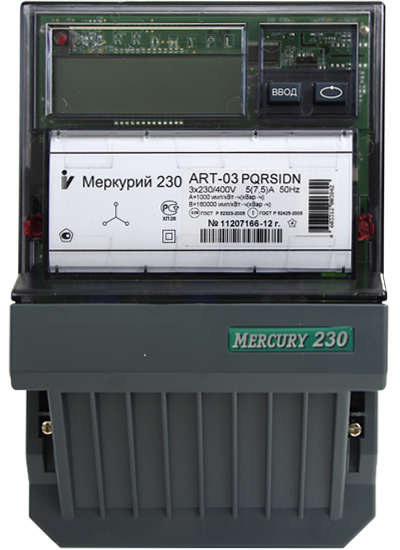
\includegraphics[scale=0.6]{img/mercury.png}
	\caption{<<Меркурий 230 ART-03>>}
\end{figure}

\newpage

\section{Протоколы}

Набор правил, позволяющий осуществлять соединение и обмен данными межджу двумя и более включёнными в сеть компьютерами, называется \textbf{сетевым протолом}.
Сами протоколы лишь описывают разные стороны одной и той же связи; взятые вместе, они образуют так называемый стек протоколов. Названия <<протокол>> и <<стек протоколов>> также указывают на программное обеспечение, которым реализуется протокол\cite{protocols}.

Распространённой системой классификации сетевых протоколов является так называемая модель OSI. В соответствии с этой моделью протоколы делятся на 7 уровней по своему назначению ~--- от физического до прикладного (см. таблицу~\ref{osi}). 

Протоколы работают друг с другом в стеке --- это означает, что протокол располагающийся на уровне выше, инкапсулируется в протокол нижнего уровня. Например, протокол UDP работает поверх протокола IP.

\begin{table}[h!]
\caption{Уровни протоколов в модели OSI}
\label{osi}
	\begin{tabular}{|c| >{\centering} m{120mm} <{\centering}|}
	\hline
	Уровень & Назначение \\
	\tabularnewline
	\hline
	Прикладной & Обеспечивает взаимодействие сети и пользователя. Уровень разрешает приложениям пользователя доступ к сетевым службам.\\
	\tabularnewline
	\hline
	Представления & Отвечает за преобразование протоколов и кодирование/декодирование данных.\\
	\tabularnewline
	\hline	
	Сеансовый & Отвечает за поддержание сеанса связи, что позволяет приложениям взаимодействовать друг с другом длительное время.\\
	\tabularnewline
	\hline
	Транспортный & Доставка данных без ошибок, потерь, дублирования и в правильной последовательности.\\
	\tabularnewline
	\hline
	Сетевой & Определение пути передачи данных. Нахождение кратчайших маршрутов.\\
	\tabularnewline
	\hline
	Канальный & Обеспечание взаимодействия сетей на физическом уровне и контроля за ошибками, которые могут возникнуть.\\
	\tabularnewline
	\hline
	Физический & Непосредственная передача потока данных через физическую среду.\\
	\tabularnewline
	\hline 
	\end{tabular}
\end{table}

\subsection{Стек протоколов TCP/IP}

\textit{Transmission Control Protocol/Internet Protocol (TCP/IP)} - это промышленный стандарт стека протоколов, разработанный для глобальных сетей\cite{tcpip}.

Этот стек протоколов был разработан до появления модели взаимодействия открытых систем. Несмотря на то, что он также имеет многоуровневую структуру, соответствие уровней стека TCP/IP уровням модели OSI весьма условно.

Работа УСПД напрямую зависит от способности поддерживать данный стек протоколов. Это объясняется следующим:
\begin{itemize}
\item Это метод получения доступа к сети Internet.
\item Это наиболее популярный и в то же время завершенный стандартный стек сетевых протоколов, имеющий многолетнюю историю
\item Все современные операционные системы поддерживают стек TCP/IP. 
\item Это устойчивая масштабируемая межплатформенная среда для приложений клиент-сервер.
\end{itemize}

\chapter{РЕАЛИЗАЦИЯ}

%-------------------------------------------------------%

\iffalse
\chapter{Требования к форме документа}

\section{Общие требования}

Отчёт может быть рукописным, но, как правило, должен быть оформлен с использованием стандартных редакторов на ЭВМ (для выпускных квалификационных работ -- обязательно) (по согласованию с руководителем во всех случаях, кроме дипломов, может представляться только электронная копия работ). Отчёт пишется (печатается) с одной стороны листа на белой бумаге формата А4 с полями не менее 10~мм справа, 30~мм слева, 20~мм сверху, 20~мм снизу. Поля не отчёркиваются. Листы должны быть сброшюрованы (отчёт переплетен, сшит, заключен в <<папку для дипломов>>).

Каждую главу отчёта следует начинать с нового листа. Листы отчёта нумеруются подряд, начиная с титульного листа (ему присваивается номер 1, однако на этом листе номер не ставится). Номер страницы проставляется в центре нижней части страницы.

Примеры оформления титульного листа приведены в \cite{dferules}.

Для отчётов по НИР и грантам, представляемым в другие организации, а также на депонирование, титульный лист содержит и другие элементы (индекс УДК, грифы согласования и утверждения, см. ГОСТ 7.32-2001).

Если отчёт состоит из двух и более книг, то на титульном листе каждой книги под указанием вида отчета указывается арабскими цифрами -- часть 1 или часть 2.

Если работа выполнена коллективом авторов, то на листе 2 помещается ``СПИСОК ИСПОЛНИТЕЛЕЙ''. Под таким заголовком в алфавитном порядке перечисляются: фамилия, инициалы исполнителя, курс (группа) для студента или должность, если в составе творческой группы есть сотрудники, и указываются разделы отчёта, в которых отражена выполненная данным исполнителем часть работы.

Если отчёт выполнен одним исполнителем, то его должность, фамилию и инициалы следует указывать на титульном листе отчёта.

\section{Структурные элементы отчета}

На следующем листе пишется слово ``Реферат'', далее указывается число страниц, таблиц, рисунков и ссылок на литературу в данной работе. Затем следует краткое изложение постановки задачи, методов её решения, основных результатов. Далее пишутся ключевые слова, перечисленные в алфавитном порядке в именительном падеже (5--10 слов, отражающих основное содержание работы). Объём реферата -- примерно $^1/_2$ страницы.

На следующем за рефератом листе (или листах) помещается содержание работы. Под заголовком ``Содержание'', написанным посередине верхней строки, помещается наименование разделов и номера страниц, с которых они начинаются.

Если в отчёте есть ссылки на стандарты, то перечень этих стандартов оформляется отдельным структурным элементом отчёта ``Нормативные ссылки'', который следует за разделом ``Содержание''.

В случае необходимости после содержания может быть помещен структурный элемент ``Определения'', который содержит определения, необходимые для уточнения или установления терминов, используемых в отчёте.

Следующий структурный элемент ``Обозначения и сокращения'' содержит перечень сокращений, условных обозначений, терминов.

Далее с нового листа начинается основной текст отчета. Отчет должен состоять из введения, разделов основной части, заключения, списка использованных источников и (при необходимости) приложений.

Каждый из разделов начинается с нового листа. Разделы нумеруются арабскими цифрами (введение и заключение не нумеруются).

Разделы могут разделяться на подразделы. Заголовки подразделов печатаются строчными буквами. Подразделы не начинают с новой страницы. Подразделы нумеруют двойной нумерацией: номер раздела, номер подраздела (после номера раздела, подраздела, пункта и подпункта точка не ставится, например ``3.2'').

\section{Оформление перечислений}

Внутри пункта или подпункта могут использоваться перечисления, которые можно оформить двумя способами: с помощью строчных букв (за исключением ё, з, о, ь, й, ы, ъ) или с помощью дефиса.

Примеры:
\begin{itemize}
\item далее текст;
\item далее текст;
\item далее текст.
\end{itemize}
\begin{enumerate}
\item далее текст;
\item далее текст;
\item далее текст.
\end{enumerate}

\section{Оформление рисунков}

Рисунки, включаемые в отчёт, могут выполняться на отдельных листах -- в этом случае они помещаются вслед за страницей, где впервые упоминается данный рисунок и страница с рисунком включается в общую нумерацию страниц. Допускается включение рисунков в текст, однако размер рисунка должен быть достаточным для чёткого восприятия его деталей и надписей.

Рисунки нумеруются подряд в пределах данного раздела двойной нумерацией: ``номер раздела.номер рисунка''.

Все рисунки снабжаются подписями независимо от того, как подробно описано в тексте отчёта то, что изображено на данном рисунке.

Слово ``Рисунок'', его номер и наименование размещают следующим образом:

\begin{figure}[h]
\centering
\begin{picture}(50,20)
\put(25,10){\oval(20,10)}
\end{picture}
\caption{Детали прибора}
\end{figure}

Чертежи и электронные схемы, помещаемые в отчёт, должны оформляться в соответствии с требованиями ЕСКД (единой системы конструкторской документации).

Все графики должны иметь на координатных осях указания отложенных величин, единиц их измерения и масштабную сетку.

\section{Оформление таблиц}

Таблицы нумеруются так же, как и рисунки. Все таблицы должны иметь содержательный заголовок, указание на проставленные по столбцам (строкам) и в клетках таблицы величины и единицы их измерения. Название таблицы следует помещать над таблицей слева без абзацного отступа в одну строку с её номером и тире. Не допускается применение диагональных линий в заголовках таблиц.

\begin{table}[h]
\caption{Коды направлений подготовки \cite{bachcodes, mastercodes}}
\begin{tabular}{|c|c|p{80mm}|}
\hline
Код & Уровень & Описание\\
\hline
05.03.01 & бакалавриат & Геология\\
09.03.01 & бакалавриат & Информатика и вычислительная техника\\
09.04.01 & магистратура & Информатика и вычислительная техника\\
11.03.04 & бакалавриат & Электроника и наноэлектроника\\
11.04.04 & магистратура & Электроника и наноэлектроника\\
12.03.01 & бакалавриат & Приборостроение\\
12.04.01 & магистратура & Приборостроение\\
13.03.01 & бакалавриат & Теплоэнергетика и теплотехника\\
13.03.02 & бакалавриат & Электроэнергетика и электротехника\\
13.04.02 & магистратура & Электроэнергетика и электротехника\\
16.03.01 & бакалавриат & Техническая физика\\
21.05.04 & специалитет & Горное дело\\
\hline
\end{tabular}
\end{table}

При большом количестве таблиц и рисунков допускается приводить их все или часть из них в приложении.

\section{Оформление приложений}

Каждое приложение следует начинать с новой страницы с указанием наверху посередине страницы слова ``Приложение'' с его обозначением с помощью заглавных букв русского алфавита (кроме Ё, З, Й, О, Ч, Ь, Ы, Ъ). Пример: ``Приложение Б''.

Приложение должно иметь заголовок, который пишется симметрично относительно текста с прописной буквы отдельной строкой. Если в отчёте одно приложение, то оно обозначается так: ``Приложение А''.

Допускается обозначение приложения буквами латинского алфавита за исключением букв I и О.

Рисунки и таблицы каждого приложения обозначаются отдельной нумерацией арабскими цифрами с добавлением перед цифрой обозначения приложения. Пример: ``Рисунок А.5'' или ``Таблица Б.2''.

\section{Оформление формул}

Формулы, на которые в дальнейшем будут ссылки, нумеруются двойной нумерацией в скобках: ``(номер раздела.номер формулы)''. Ссылки на формулы даются так же в скобках. Формулы, как правило, следует выделять в отдельную строку (нумерованные обязательно выделять в отдельную строку).

\begin{equation}\label{fourier}
\hat{f}(\omega)=\frac{1}{\sqrt{2\pi}}\int\limits_{-\infty}^{\infty}f(x)e^{-ix\omega}\,dx.
\end{equation}

В формуле \eqref{fourier} указаны: $f(x)$ -- исходная функция, $\hat{f}(\omega)$ -- её Фурье-образ.

\section{Оформление библиографии}

Список литературы дается в конце работы (перед приложениями) под заголовком ``Список использованных источников''.

Сведения об источниках следует располагать в порядке появления ссылок на источники в тексте отчёта и нумеровать арабскими цифрами без точки и печатать с абзацного отступа.

В основном тексте ссылки на использованные источники следует приводить в квадратных скобках.

Оформление элементов списка литературы должно соответствовать приведённым в приложении примерам.

При ссылке в тексте отчёта на стандарты или технические условия указывают только их обозначения (при этом допускается не указывать год их утверждения) при условии полного описания стандарта в списке использованных источников.

%\section{Оформление примечаний}

%Если примечание одно, то оно оформляется так: Примечание --- далее текст. Если несколько:

%Примечания
%1 далее текст
%2 далее текст. 

\chapter{Требования к содержанию работы}

\section{Требования к введению}

Во введении излагается цель и назначение работы, обосновывается её актуальность, даётся оценка современного состояния решаемой проблемы, указывается на возможные области внедрения. Может быть приведено задание на работу. Может быть сделан краткий обзор отчёта, обоснована его структура (особенно, если взаимосвязь его разделов на первый взгляд не очевидна). Введение должно быть кратким (2--3 стр.). Из введения читатель должен понять основную цель и содержание работы. Это как бы реклама работы и отчёта. Читатель, впервые взявший отчёт и не знакомый с работой, прочитав введение, должен понять, стоит ли читать дальше.

\section{Требования к основной части}

Проприетарное ПО - программное обеспечение, являющееся частной собственностью авторов или правообладателей и неудовлетворяющее критериям свободного программного обеспечения.

Критерии свободного ПО по Ричарду Столлману: (источник Википедия)

0. Свобода запускать программу в любых целях.

1. Свобода изучения работы программы и адаптация ее вашим нуждам (доступ к исходным текстам является необходимым условиям)

2. Свобода распространять копии, так что вы можете помочь вашему товарищу.

3. Свобода улучшать программу и публиковать ваши улучшения, так что все общество выиграет от этого (доступ к исходным текстам является необходимым условием)

В первом разделе, который обычно называют ``Аналитический обзор'', ``Патентно"=литературный обзор'' (но можно и иначе) содержатся результаты предварительных исследований (они могут занять и более одного раздела, если носят разносторонний характер).

Разделы, содержащие результаты предварительных исследований, должны завершаться постановкой задачи. Постановку задачи следует изложить в отдельном разделе или, по крайней мере, чётко выделить в тексте отдельным абзацем.

В литературном обзоре следует избегать прямого пересказа рассматриваемых работ и воспроизведения рисунков из них. Надо по возможности обобщать и анализировать их результаты в той мере, в какой они имеют отношение к выполняемой работе. Цитировать, воспроизводить выкладки следует только тогда, когда это имеет принципиальное значение для постановки задачи или выбора метода её решения в выполняемой работе. Текстовые цитаты следует заключать в кавычки. Все заимствования сопровождаются ссылками на литературу. Текст отчета должен позволить читателю однозначно отделить заимствования из литературы от собственных выводов, оценок, предложений автора работы.

Если работа не ставится как чисто реферативная, то обзор литературы должен составлять по объёму не более $^1/_5$\,--\,$^1/_4$ всего отчёта.

В разделах, отражающих основную часть работы, следует описывать её максимально полно и подробно.

При описании экспериментов, измерительных или технологических, надо приводить сведения о всех контролируемых параметрах эксперимента (процесса), даже если эти сведения кажутся исполнителю не имеющими прямого отношения к решаемой задаче. Следует указывать способы контроля параметров (приборы) и приводить сведения об их метрологической аттестации.

При описании конструкторских разработок, изготовлении макетов, приборов, образцов для исследования следует не только описывать окончательный результат (установку, образец), но и технологию его получения.

При выборе экспериментальных и теоретических методов решения задачи и конструкторских или программных решений следует подробно обосновывать сделанный выбор как на основе литературного обзора, так и на основе проделанных экспериментов. В частности, следует описывать и анализировать все опробованные методы и конструкции, даже если они отвергнуты в окончательном варианте работы.

Если в работе выполнялись какие-либо измерения и (или) расчеты, то следует приводить (с указанием погрешности!) не только их окончательные результаты, но и по возможности все промежуточные результаты (непосредственные результаты измерений, использованные в последующих расчётах табличные и другие дополнительные данные; результаты всех повторных измерений, расчётов, результаты, полученные при различных вариантах измерительной (расчётной) методики и т.\,д. (однако можно это делать и в приложении).

Во всех формулах, приводимых в отчёте, следует расшифровать смысл входящих в них величин и указывать единицы их измерения непосредственно после формул. (При последующих использованиях той же буквы в том же смысле её можно не расшифровывать). Допускается приводить единый ``Список обозначений'' (с указанием единиц измерения). Он помещается после содержания.

Основную часть работы следует писать так, чтобы читатель, обладающий квалификацией исполнителя, но ранее не знакомый с работой мог бы, при наличии в его распоряжении перечисленного в тексте работы оборудования, материалов и вычислительных средств, действуя по описанным методикам без каких-либо дополнительных исследований, расчётов и разработок и без обращения к справочной и иной литературе воспроизвести результат работы.

\section{Рекомендации к содержанию приложений}

В приложения выносятся громоздкие по объёму материалы, наличие которых в основном тексте затруднило бы его восприятие:
\begin{itemize}
\item таблицы промежуточных результатов и других вспомогательных данных,
\item рисунки, если количество их велико,
\item подробные электрические схемы,
\item тексты и описания программ для ЭВМ.
\end{itemize}

\section{Требования к описанию разработанных программ}

Описание программы должно включать:
\begin{itemize}
\item Название и назначение программы.
\item Язык программирования и название компилятора.
\item Требования к технической и программной среде для её функционирования (аппаратная платформа, процессор, ОС, объемы памяти, дополнительные требования и т.\,п.).
\item Описание алгоритма и структуры (математическая основа, логическая схема, процедуры и т.\,д.). При наличии подробных комментариев в листинге описание может быть кратким. Этот раздел может быть дополнен пояснениями, не касающимися структуры программы, но являющимися важными для понимания её работы.
\item Описание используемых ключевых переменных (возможно непосредственно в самом листинге программы).
\item Перечень используемых библиотечных функций.
\end{itemize}

Разработанная программа должна сопровождаться инструкцией пользователя (как запустить программу, что и в каком формате вводить, формат файлов входных и выходных данных и т.\,д. Опять же подробность этого раздела зависит от качества интерфейса. Важно, чтобы для работы программы не требовалось присутствия автора и пользователь не должен был разбираться в исходных текстах). Очень желательно, чтобы инструкция была встроена внутрь программы.

Если есть необходимость, инструкция пользователя сопровождается примером действия программы.

Исходные тексты и скомпилированный экземпляр программы обязательно должны прилагаться к тексту защищаемой работы на электронном носителе. 

\chapter{Дополнительные требования к квалификационным работам
(бакалаврским, дипломным, магистерским)}

Работа должна представлять собой законченную научно-исследовательскую, проектную или технологическую разработку, в которой решается актуальная задача выбранного направления профессиональной деятельности.

Если целью работы является создание программного продукта или прибора, в работу включается в качестве самостоятельных разделов:
\begin{itemize}
\item техническое задание на проектируемый объект;
\item экономический раздел, в котором обсуждается стоимость продукта, маркетинг, возможности рекламы;
\item раздел обеспечения безопасности жизнедеятельности, если в процессе или результате разработки могут возникнуть какие-либо факторы, опасные для человека или окружающей среды.
\end{itemize}

\fi

\backmatter %% Здесь заканчивается нумерованная часть документа и начинаются заключение и ссылки

\Conclusion

В заключении кратко излагаются основные результаты работы, оценивается степень достижения поставленной цели. Могут даваться рекомендации по дальнейшему развитию работы и возможным применениям полученных результатов. Из заключения читатель должен увидеть объём проделанной работы и её ценность.

%% Альтернативное оформление библиографического списка:
\begin{thebibliography}{99}

\bibitem{qualitymonitor} Монитор качества электроэнергии. [Электронный ресурс] /  Режим доступа: http://fidercom.ru/pribory-uchyota-elektroenergii/monitoring-kachestva-\\elektroenergii.html. --- (Дата последнего обращения: 13.05.2017).

\bibitem{ascaepinfo} Автоматизированная система коммерческого учета электроэнергии (АСКУЭ). / Н.М. Гришагина, Э.Г Гарайшина. // Вестник Казанского технологического университета. --- 2013. --- \No~12. --- С.~297-299.

\bibitem{ethernetinfo} Что такое Ethernet / Всё о компьютерных сетях. [Электронный ресурс] ~--- 2010. ~--- Режим доступа: http://loknet.ru/teoriya/chto-takoe-ethernet.html --- (дата последнего обращения: 13.05.2017)

\bibitem{ethersite2} Технология Ethernet. Обзор технологии. Разновидности Ethernet. Стандарты Ethernet. / Инсотел - Поставки сетевого и серверного оборудования. [Электронный ресурс] ~--- URL: http://www.insotel.ru/article.php?id=240 --- (дата последнего обращения: 13.05.2017)

\bibitem{gsmwiki} GSM / Википедия. [Электронный ресурс] ~--- Режим доступа: https://ru.wikipedia.org/wiki/GSM --- 2017. --- (дата последнего обращения: 13.05.2017)

\bibitem{gsmchar} Общая характеристика стандарта GSM [Электронный ресурс] ~--- URL: http://life-prog.ru/2\_77781\_obshchaya-harakteristika-standarta-GSM.html  --- 2015. --- (дата последнего обращения: 13.05.2017)

\bibitem{wifistandarts} Wi-Fi, Стандарты [Электронный ресурс] ~--- Режим доступа: http://wi-life.ru/texnologii/wi-fi/wi-fi-standarty --- (дата последнего обращения: 13.05.2017)

\bibitem{mercinfo1} Краткое описание устройства и принципа действия счетчика меркурий 230. [Электронный ресурс] ~--- Режим доступа: http://libdocs.ru/docs/141100/index-429.html --- (дата последнего обращения: 13.05.2017)

\bibitem{mercinfo2} СЧЁТЧИКИ ЭЛЕКТРИЧЕСКОЙ ЭНЕРГИИ 
трёхфазные, активно/реактивные, многофункциональные. [Электронный ресурс] ~--- Режим доступа: http://www.incotexcom.ru/m230art.htm --- (дата последнего обращения: 13.05.2017)

\bibitem{protocols} Что такое сетевой протокол? / Компания АВК [Электронный ресурс] ~--- Режим доступа: https://www.avk-company.ru/articles/25/ --- (дата последнего обращения: 13.05.2017)

\bibitem{tcpip} Стек протоколов TCP/IP / CITFORUM [Электронный ресурс] ~--- Режим доступа: http://citforum.ru/nets/ip/glava\_2.shtml --- (дата последнего обращения: 13.05.2017)

\end{thebibliography}

%% Оформление библиографического списка при помощи BibTeX:
%\bibliographystyle{ugost2003} % <-- avsolov: это стандартный стиль
%\bibliography{research_report} % подключаем файл research_report.bib

\appendix

\chapter{Исходные тексты программ}

%-------------------------------------------------------------->> КОНЕЦ
\iffalse




\chapter{Образцы библиографического описания документов}

Следующие образцы оформлены в соответствии с ГОСТ 7.1-2003. Строгое соответствие данному ГОСТ требуется при оформлении каталожных карточек, библиографических списков депонируемых отчётов и диссертаций, отправляемых в ВАК. 

Разрешается в курсовых и ВКР оформлять элементы библиографического списка как библиографические ссылки по ГОСТ Р 7.0.5-2008, который допускает:
\begin{itemize}
\item не ставить запятую после фамилии автора;
\item не использовать тире для разделения элементов библиографического описания;
\item опускать элементы, не влияющие на идентификацию произведения.
\end{itemize}

~

Например, полное описание по ГОСТ 7.1-2003:\\
Авдеев, Н. А. Твердотельная электроника : учеб. пособие для студентов техн. и
инж. специальностей и аспирантов / Н. А. Авдеев ; М-во образования и науки Рос. Федерации, Федер. гос. бюджет. образоват. учреждение высш. проф. образования
Петрозавод. гос. ун-т. --- Петрозаводск : Изд-во ПетрГУ, 2013. --- 58 с. : ил.

~

Библиографическая ссылка по ГОСТ Р 7.0.5-2008:\\
Авдеев Н. А. Твердотельная электроника : учеб. пособие для студентов техн. и
инж. специальностей и аспирантов. Петрозаводск : Изд-во ПетрГУ, 2013. 58 с.

~

Пример описания книги с двумя авторами:\\
Лайдинен, Э. П. Финская разведка против Советской России : специальные
службы Финляндии и их разведывательная деятельность на Северо-Западе России,
1914--1939 гг.~/ Э.\,П.\,Лайдинен, С.\,Г.\,Веригин. --- Изд. 2-е, доп. и испр. --- Петрозаводск : Verso, 2013. --- 295~с.~: ил.

~

Пример описания книги с тремя авторами:\\
Муллонен, И. И. Свод топонимов Заонежья / И. И. Муллонен, И. В. Азарова, А. С. Герд~; под ред. А. С. Герда ; Рос. акад. наук, Карел. науч. центр, Ин-т яз., лит. и истории, С.-Петерб. гос. ун-т. --- Петрозаводск, 2013. --- 250 с. : ил., карты.

~

Пример описания книги с большим количеством авторов:\\
Онежское озеро / Г. С. Бискэ, С. В. Григорьев, Т. И. Малинина, А. Ф. Смирнов, Е.\,М.\,Эп\-штейн~; [науч. ред. Г. С. Бискэ]. --- Петрозаводск : Карелия, 1975. --- 163, [3] с.~: фот. --- Библиогр.: с. 165.\\
Или:\\
Онежское озеро / Г. С. Бискэ [и др. ; науч. ред. Г. С. Бискэ]. --- Петрозаводск : Карелия, 1975. --- 163, [3] с. : фот. --- Библиогр.: с. 165.

~

Пример описания статьи из сборника:\\
Веригин, С. Г. <<Карельский вопрос>> в национальной политике финских оккупационных властей в Восточной Карелии в 1941--1944 гг. / С. Г. Веригин // Карелы российско-финского пограничья в XIX--XX вв. : сб. ст. / М-во образования и науки Рос. Федерации, Федер. гос. бюджет. образоват. учреждение высш. проф. образования «Петрозавод. гос. ун-т» ; [отв. ред. А. М. Пашков]. --- Петрозаводск, 2013. --- С. 212--235. 

~

Пример описания статьи из журнала:\\
Айгистов, Р. А. Современный книжный рынок России / Р. А. Айгистов // Библиография.~--- 2014. --- \No~4. --- С. 3--10.

~

Пример описания статьи из газеты:\\
Куроптев, В. Повышение квалификации в области разработки и создания наноэлектронной продукции / В. Куроптев // Петрозаводский университет. --- 2014. --- 5 сент. --- С.~3.

~

Пример описания статьи из продолжающегося издания:\\ 
Тарасов, К. Г. Дания и Швеция в <<Дневном журнале...>> В. И. Даля / К.\,Г.\,Тарасов, А.\,О.\,Сухов // Учен. зап. Петрозавод. гос. ун-та. Сер.: Общественные и гуманитарные науки. --- 2014. --- \No~1 (138). --- С. 67--69. 

~

Пример описания стандарта:\\
ГОСТ 31168-2014. Здания жилые. Метод определения удельного потребления тепловой энергии на отопление. -- Взамен ГОСТ 31168-2003 ; введ. 2015-01-01. --- Москва : Стандарт-Информ, 2014. --- 18 с. --- (Межгосударственный стандарт).

~

Пример описания патента:\\
Патент 130865 Рос. Федерация, МПК A 63 B 22/18. Устройство для тренировки вестибулярного аппарата спортсменов / И. Р. Шегельман, А. В. Демчук ; патентообладатель Петрозавод. гос. ун-т. --- \No~2013112039/12 ; заявл. 18.03.2013 ; опубл. 10.08.2013, Бюл. \No~22.~--- 2 с. : ил. 

~

Пример описания авторского свидетельства:\\
Авт. свид. 1261797 СССР, МКИ$^4$ B 27 L 1/00. Лесозаготовительная машина / И.\,Р.\,Шегель\-ман, Г.\,П.\,Зайцев, Э.\,Э.\,Мейер ; заявитель Kаpeл. научно-исслед. ин-т 
лесной пром-сти. --- \No~3923668/29-15 ; заявл. 12.05.85 ; опубл. 07.10.86, Бюл. \No~37. --- 4 с. : ил. 

~

Пример описания свидетельства о госрегистрации базы данных:\\
Свидетельство о госрегистрации базы данных \No~2013620592 Рос. Федерация.
<<Okorka -- база данных по учету РИД>> / И. Р. Шегельман, А. С. Васильев, Ю. В. Суханов ; правообладатель Петрозавод. гос. ун-т. --- \No~2013620238~; заявл. 12.03.2013~; зарегистр. 07.05.2013~; опубл. 20.06.2013. --- 1 с. 

~

Пример описания диссертации:\\
Белякова, Е. Н. Биологические особенности молоди лососевых рыб в реках Карелии и Кольского полуострова : дис. ... канд. биол. наук : 03.02.06 / Белякова Елена Николаевна.~--- Петрозаводск, 2013. --- 137 с. : ил., табл. --- Библиогр.: с. 125--137 (129 назв.)

~

Пример описания автореферата диссертации:\\
Воронцова, М. Г. Стратегия развития российской системы управления образованием в области туризма : автореф. дис. ... д-ра экон. наук : 08.00.05 / Воронцова Маргарита Гурьевна ; С.-Петерб. ун-т экономики и финансов. --- Санкт-Петербург, 2004. --- 37 с.

~

Пример описания электронной статьи:\\
Гарскова, И. М. Источниковедческие проблемы исторической информатики [Электронный ресурс] / И. М. Гарскова. --- Электрон. ст. --- [Россия], 2010. --- Режим доступа: http://aik-sng.ru/node/265, свободный. --- Аналог печ. изд. (Российская история. --- 2010.~--- \No~3. --- С. 151--161). --- (20.04.2015). 

~

Пример описания электронных данных (веб-сайт и т.\,д.):\\
eLibrary.karelia.ru [Электронный ресурс] : электронная библиотека Республики 
Карелия~/ Петрозавод. гос. ун-т [и др.]. --- Электрон. дан. --- [Петрозаводск], cop. 1998. --- Режим дос\-тупа: http://elibrary.karelia.ru. --- (20.04.2015). 

~

Пример описания составной части электронного ресурса:\\
Кириков Б. М. Модерн / Б. М. Кириков // Санкт-Петербург [Электронный ресурс] : энциклопедия / [упр. и развитие проекта Междунар. благотворит. фонд им. Д. С. Лихачева, Ин-т Петра Великого ; рук. проекта А. Кобак ; прогр.-технолог. комплекс ОАО 
<<Альт-Софт>> ; дизайнер А. Опочанский]. --- Электрон. дан. --- [Санкт-Петербург], [2015]. --- URL: http://www.encspb.ru/object/2804006741?lc=ru. --- (20.04.2015).

~

Пример описания законодательных материалов:\\
О государственном кадастре недвижимости : Федер. закон от 24.07.2007~г. \No~221-ФЗ : принят Гос. Думой 4 июля 2007 г. : одобр. Советом Федерации 11 июля 2007 г. // КонсультантПлюс [Электронный ресурс] : справ. прав. система / Компания <<КонсультантПлюс>>.~--- Электрон.  дан. --- [Москва],  cop. 1997. --- URL: http://www.consultant.ru. --- (20.04.2015). 

~

Некоторые пояснения по формату библиографического описания:

В квадратных скобках даются сведения, явно не указанные на титульном листе произведения, но которые можно определить из контекста или последующих листов. 

Популярные сокращения: <<б.\,м.>> -- без места (место издания неизвестно), <<б.\,и.>>~-- без издательства (издательство неизвестно), <<б.\,г.>> -- без года (год издания неизвестен). <<cop.>> -- copyright (дата присвоения авторского права). Полный список допустимых сокращений есть в ГОСТ Р 7.0.12-2011.

Вместо <<режим доступа>> допускается писать <<URL>>.

Знаки-разделители элементов библиографического описания (--- ; :) отбиваются пробелами  с обеих сторон.

\chapter{Особенности использования \LaTeX{} для оформления ВКР}

\section{Общие сведения}

\LaTeX{} -- популярный набор макропакетов для системы компьютерной вёрстки \TeX. Ознакомиться с возможностями \LaTeX{} можно, например, при помощи учебника \cite{latex}.

Для удобства студентов подготовлена модификация \LaTeX{}"=класса документов G7-32, позволяющая оформлять выпускные квалификационные работы, отчёты по производственной и учебной практике, по научно-исследовательской и курсовой работе студентов.

Актуальная версия класса размещена по адресу:

https://dims.karelia.ru/svn/g7-32/

Для оформления нового документа необходимы файлы:
\begin{itemize}
\item G7-32.cls -- описание класса документа G7-32;
\item G7-32.sty -- описание стилевого пакета G7-32 (используется классом G7-32);
\item G2-105.sty -- описание стилевого пакета G2-105 (используется классом G7-32).
\end{itemize}

Кроме того, по этому адресу размещён адаптированный стилевой пакет \texttt{ugost2003} для Bib\TeX{} (файлы ugost2003.bst, gost.dtx, gost.ins, utf8cyrillic.csf).

Данные <<Правила...>> содержатся в файле thesis.tex. Остальные TEX-файлы содержат примеры титульных листов.

\section{Преамбула документа}

Документ класса G7-32 в опциях, кроме кодировки и стандартного размера шрифта, должен содержать обозначение вида документа:
\begin{itemize}
\item \texttt{masterthes} -- диссертация магистра;
\item \texttt{diploma} -- дипломная работа инженера;
\item \texttt{bachelor} -- квалификационная работа бакалавра;
\item \texttt{coursreport} -- курсовая работа;
\item \texttt{projreport} -- курсовой проект по дисциплине;
\item \texttt{appreport} -- отчет о прикладных научных исследованиях;
\item \texttt{scireport} -- отчет о научно-исследовательской работе;
\item \texttt{report} -- отчёт (по практике).
\end{itemize}

Например:
\begin{verbatim}
\documentclass[utf8,12pt,masterthes]{G7-32}
\end{verbatim}

Далее после подключения необходимых стилевых пакетов могут следовать команды:
\verb|\TableInChapter|, \verb|\PicInChapter|, \verb|\EqInChapter|. Эти команды определяют двухуровневую нумерацию, соответственно, таблиц, рисунков и формул. ГОСТ допускает также одноуровневую (сквозную) нумерацию таких объектов. Если применяется одноуровневая нумерация, эти команды в преамбуле отсутствуют.

Командой \verb|\NirOrgLongName| определяется наименование организации, в которой выполняется работа. Текстовый параметр этой команды появится в верхней части титульного листа документа.

Для формирования разлиновки под подписи на титульном листе используется макрос \verb|\signfield| с двумя параметрами. Первый параметр -- должность и регалии лица, второй параметр -- фамилия и инициалы. При необходимости первый параметр может состоять из нескольких строк, разделяемых командой \verb|\newline|.

Например, команда:
\begin{verbatim}
\signfield{Главный начальник:}{И.\,И.\,Иванов}
\end{verbatim}
формирует такую разлиновку:
\begin{center}
\signfield{Главный начальник:}{И.\,И.\,Иванов}
\end{center}

Макрос \verb|\signfield| используется как параметр для команд, формирующих разлиновку под визы на титульном листе. В выпускных квалификационных работах предусмотрено две визы: виза автора (команда \verb|\NirAuthor|) и виза научного руководителя (команда \verb|\NirSupervisor|).

Кроме того, на титульном листе указывается также место выпуска документа (команда \verb|\NirTown|) и год выпуска (команда \verb|\NirYear|). Если команда \verb|\NirYear| не указана, подставляется текущий год.

\section{Структура основной части документа}

Основная часть документа (окружение document) имеет следующую структуру:
\begin{flushleft}
\verb|\begin{document}|\\
\verb|\frontmatter|\\
Сервисные (ненумеруемые разделы отчёта: реферат, содержание, введение и т.\,п.\\
\verb|\mainmatter|\\
Основные разделы отчёта.\\
\verb|\backmatter|\\
Заключение и список литературы.\\
\verb|\appendix|\\
Приложения.\\
\verb|\end{document}|\\
\end{flushleft}

Начинается документ с команды \verb|\frontmatter|. Эта команда временно отключает нумерацию глав.

После неё необходимо использовать макрос \verb|\NirTitle|, который задаёт название отчёту и формирует титульный лист. Первый параметр этого макроса -- название отчёта. Для многих видов отчётов в этом макросе возможен также второй параметр, который определяет дополнительный текст в строке под видом отчёта. Например, в ВКР второй параметр определяет текст направления подготовки или специальности:
\begin{verbatim}
\NirTitle{Тема ВКР}{Код Направление}
\end{verbatim}

В отчётах по практике во втором параметре можно указать вид практики:
\begin{verbatim}
\NirTitle{Название отчета}{по производственной практике}
\end{verbatim}

Команды, начинающие тот или иной сервисный раздел, указаны в табл.\,\ref{srvmacros}.

\begin{table}[h]
\caption{Команды сервисных разделов отчёта}\label{srvmacros}
\begin{tabular}{|l|p{120mm}|}
\hline
Команда & Описание\\
\hline
\verb|\Referat| & ``Реферат'' (можно использовать окружение \texttt{abstract})\\
\hline
\verb|\Executors| & ``СПИСОК ИСПОЛНИТЕЛЕЙ''\\
\hline
\verb|\tableofcontents| & ``Содержание''\\
\hline
\verb|\NormRefs| & ``Нормативные ссылки''\\
\hline
\verb|\Defines| & ``Определения''\\
\hline
\verb|\Abbreviations| & ``Обозначения и сокращения''\\
\hline
\verb|\Introduction| & ``Введение''\\
\hline
\verb|\Conclusion| & ``Заключение''\\
\hline
\end{tabular}
\end{table}

После раздела ``Введение'' должна следовать команда \verb|\mainmatter|. Эта команда включает обычную нумерацию объектов документа (разделов, рисунков, таблиц и проч.).

Разделы содержательной части отчёта задаются командами \verb|\chapter|. Следующие по иерархии рубрики (как и в прочих классах документов \LaTeX{}): \verb|\section|, \verb|\subsection|, \verb|\subsubsection|, \verb|\paragraph|.

Перед разделом ``Заключение'' следует отключить нумерацию разделов при помощи команды \verb|\backmatter|.

Список использованных источников можно формировать вручную при помощи обычного окружения \texttt{thebibliography} либо подключив соответствующий Bib\TeX{}-файл командой \verb|\bibliography|. Рекомендуемый стилевой пакет для Bib\TeX{} -- \texttt{ugost2003}.

Если в отчёте имеются приложения, после списка литературы указывается команда \verb|\appendix| и далее следуют разделы приложений.

\fi

\end{document}
